\section{Pipeline}
\label{sec:pipeline}

Eine schematische \"Ubersicht der in diesem Projekt eingesetzten
zweistufigen Vorhersagepipeline ist in Abbildung~\ref{fig:pipeline}
dargestellt.

Die Pipeline ist so aufgebaut, dass auf eine Bildeingabe zun\"achst
eine Bildsegmentierung angewendet wird, um den Bereich des Bildes,
welcher das Nummernschild enth\"alt, herauszutrennen.
F\"ur die Bildsegmentierung wurde ein CNN trainiert.
Die Einzelheiten hierzu werden in Abschnitt~\ref{sec:bildsegmentierung}
n\"aher beschrieben.

Nach der Bildsegmentierung wird auf den herausgetrennten Bereich eine
Texterkennung angewendet, um die Zeichenfolge des Nummernschildes
zu extrahieren. Dieses Verfahren wird in Abschnitt~\ref{sec:texterkennung}
beschrieben.

\begin{figure}
    \centering
    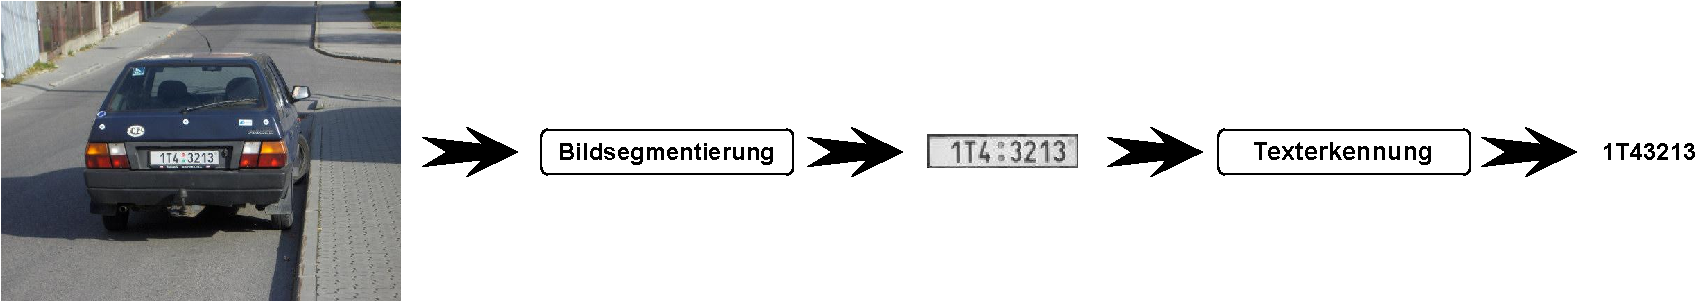
\includegraphics[width=\textwidth]{abbildungen/pipeline}
    \caption[Pipeline]{Schematische Darstellung der zweistufigen Vorhersagepipeline.
        Zun\"achst wird das Nummernschild mithilfe von Bildsegmentierung
        extrahiert. Anschlie{\ss}end werden die Zeichen durch Texterkennung
        ausgelesen.}
    \label{fig:pipeline}
\end{figure}

\subsection{Bildsegmentierung}
\label{sec:bildsegmentierung}

Das Ziel einer Bildsegmentierung ist es, die relevanten Bereiche eines
Bildes von den restlichen zu trennen.
In dieser Situation ist es also gefordert, den Bereich des Bildes,
welcher das Nummernschild enth\"alt, vom Rest des Bildes zu trennen.

Zu diesem Zweck kommt in diesem Projekt eine bin\"are Klassifikation
zum Einsatz: F\"ur jeden Pixel des Eingabebildes wird klassifiziert,
ob er Teil des Nummernschildes ist, oder nicht.
Das Ziel ist es also, f\"ur ein Eingabebild eine bin\"are Maske vorherzusagen,
welche f\"ur jeden Pixel eine 1 enth\"alt, falls er Teil des Nummernschildes
ist und anderenfalls eine 0.
Eine visuelle Darstellung dieses Konzeptes ist in
Abbildung~\ref{fig:binaere-maske} gegeben.

\begin{figure}
    \centering
    \begin{subfigure}{0.495\textwidth}
        \centering
        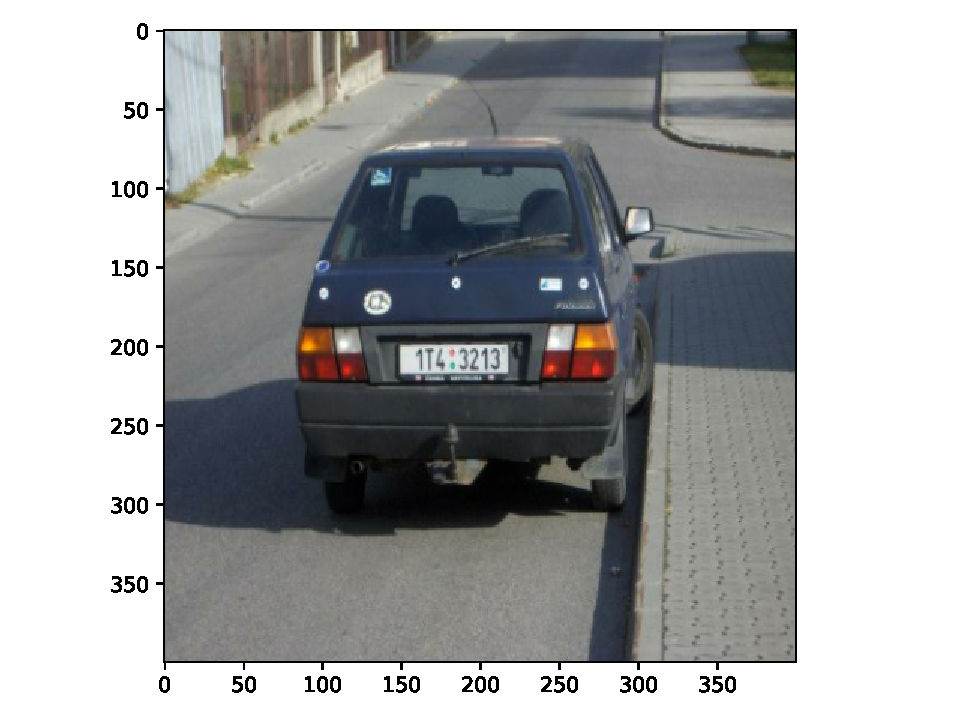
\includegraphics[width=\textwidth]{abbildungen/segmentation_input}
        \caption{Eingabebild}
    \end{subfigure}
    \begin{subfigure}{0.495\textwidth}
        \centering
        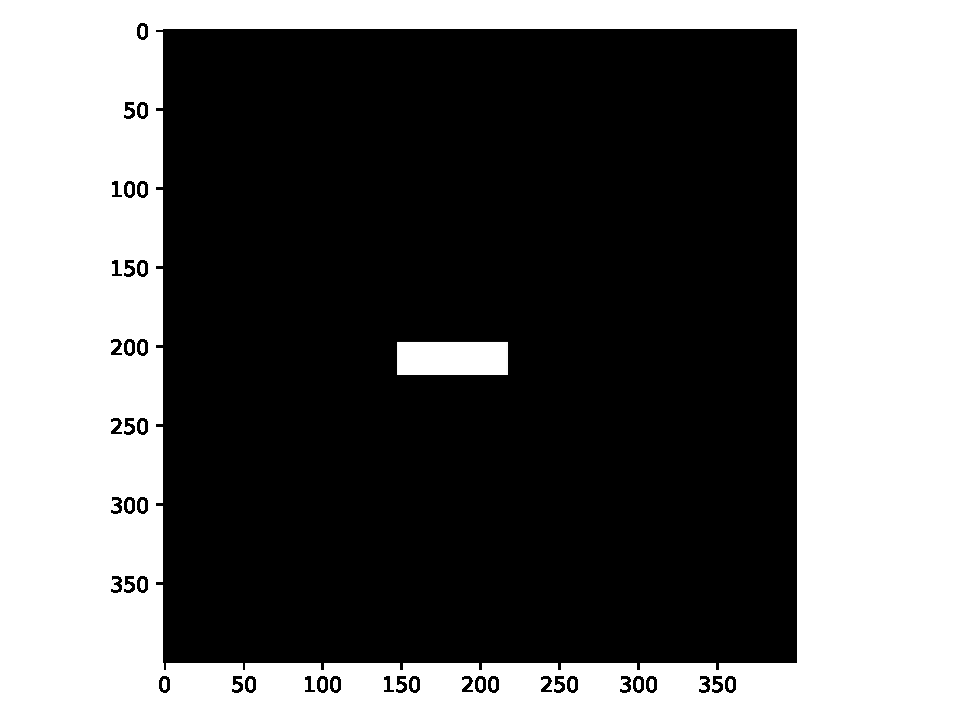
\includegraphics[width=\textwidth]{abbildungen/segmentation_output}
        \caption{Bin\"are Maske des Nummernschildes.}
    \end{subfigure}
    \caption[Bin\"are Maske]{Die bin\"are Maske (rechts) ordnet jedem Pixel der Eingabe
        (links) einen Wert 1 (hier wei{\ss} dargestellt) zu, falls sich dieser
        im Nummernschild befindet. Andernfalls wird ein Wert von 0 (schwarz)
        zugeordnet.}
    \label{fig:binaere-maske}
\end{figure}

Als Klassifikationsverfahren kommen zu diesem Zweck CNNs zum Einsatz,
die bereits in Abschnitt~\ref{sec:cnns} beschrieben wurden.
Auf die genaue Architektur und das Training des Netzes soll nun genauer
eingegangen werden.
Der Ansatz, CNNs zur Bildsegmentierung zu verwenden, geht
auf~\cite{image-segmentation} zur\"uck und wurde hier f\"ur die
vorliegende Problemstellung adaptiert.

\subsubsection{Netzarchitektur}

Wie schon in Abschnitt~\ref{sec:neuronale-netze} erl\"autert, ordnen
neuronale Netze einer Eingabe fester Gr\"o{\ss}e eine zugeh\"orige
Ausgabe fester Gr\"o{\ss}e zu.
In diesem Fall soll die Ausgabe des Netzes zu einem Eingabebild
genau die bin\"are Maske sein, welche das Nummernschild repr\"asentiert.
Da die Bilder im Datensatz allerdings verschiedene Aufl\"osungen
und damit auch verschiedene Gr\"o{\ss}en aufweisen, neuronale Netze
aber auf eine feste einheitliche Gr\"o{\ss}e angewiesen sind,
m\"ussen die Bilder vor der Eingabe in das neuronale Netz
zun\"achst auf eine einheitliche Gr\"o{\ss}e gebracht werden.
In diesem Projekt wird zu diesem Zweck jedes Bild vor der Eingabe
in das Netz auf eine Gr\"o{\ss}e von 400x400 skaliert.

Die komplette Netzarchitektur, die in diesem Projekt zum Einsatz kam,
ist in Abbildung~\ref{fig:netzarchitektur} schematisch dargestellt.
Genaue Details zu jeder Schicht, sowie die Anzahl der trainierbaren
Parameter, k\"onnen Tabelle~\ref{tab:netzarchitektur} entnommen werden.

Bei der groben Struktur der Netzarchitektur wurde sich hierbei
an~\cite{image-segmentation} orientiert. Beispielsweise ist es
zur Reduktion der trainierbaren Parameter sinnvoll, die Dimension der
Faltungsschichten zuerst schrittweise durch Pooling-Schichten zu
verkleinern und erst am
Ende wieder durch Upsampling-Schichten zu vergr\"o{\ss}ern.
Wie man in Abbildung~\ref{fig:netzarchitektur} sehen kann, verlaufen
die Ausgabedimensionen der Schichten also frei gesprochen von
\glqq breit und flach\grqq{} zu \glqq schmal und tief\grqq{} im Inneren
des Netzes und dann wieder zu \glqq breit und flach\grqq{} hin zur
Ausgabe der Vorhersage f\"ur die bin\"are Maske.

W\"ahrend sich diese allgemeine Struktur zwar generell zur Bildsegmentierung
etabliert hat, so wurde diese spezielle Architektur jedoch erst nach
vielen Testl\"aufen und Abw\"agungen gefunden. Des Weiteren scheint
die Gesamtanzahl der trainierbaren Parameter von 191.297 zwar auf den
ersten Blick sehr gro{\ss} zu sein, allerdings darf man nicht vergessen,
dass ein einziges Bild schon aus $400 \cdot 400 \cdot 3 = 480.000$
Farbwerten besteht. Die Anzahl der Parameter dieser Architektur ist also
wesentlich kleiner, als die Dimension der Modelleingabe.
Auch wenn die Netzarchitektur also als recht komplex anmutet, so ist sie
was die Zahl der freien Parameter betrifft, sogar weniger komplex als ein
lineares Modell.

Abschlie{\ss}end sei noch ein kleines, aber spannendes
Detail zur Ausgabeschicht erw\"ahnt.
Die Ausgabeschicht ist eine Faltungsschicht mit einem Kernel der
Gr\"o{\ss}e 1x1, welche die Sigmoidfunktion zur Bestimmung der
Netzausgabe verwendet. Sie enth\"alt also 9 trainierbare Parameter
(8 gehen auf den Kernel zur\"uck und 1 Parameter ist der Bias).
Sieht man genauer hin, so entspricht dies genau dem Modell
der logistischen Regression, welches als Features genau die Ausgabe
der vorherigen Faltungsschicht verwendet.
Im Grunde ist diese Netzarchitektur also eine logistische Regression, die
gleichzeitig mit einer eingebauten Feature-Extraktion trainiert wird.

\begin{figure}
    \centering
    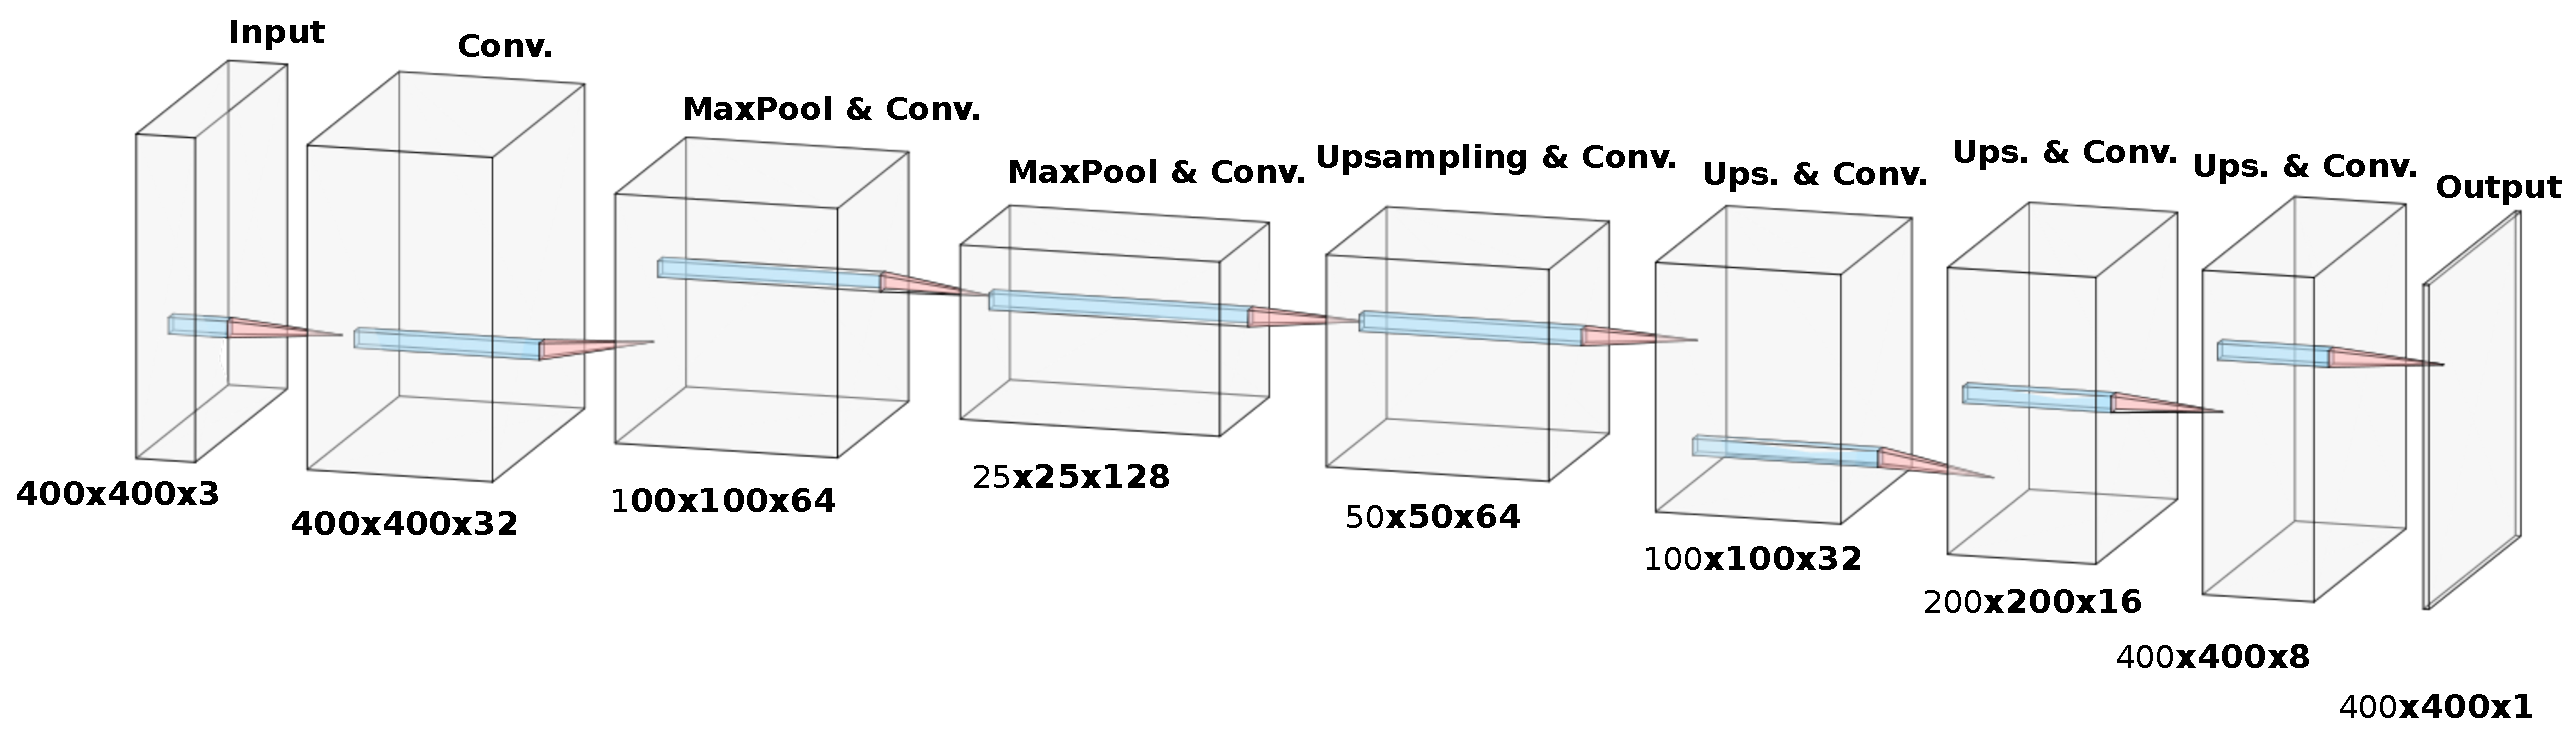
\includegraphics[width=\textwidth]{abbildungen/network_architecture}
    \caption[Netzarchitektur]{Schematische Darstellung der gew\"ahlten Netzarchitektur
    zur Bildsegmentierung. Die Eingabe des Netzes ist ein Tensor
    der Gr\"o{\ss}e 400x400x3, der das Eingabebild repr\"asentiert.
    Die Ausgabe ist eine Vorhersage der bin\"aren Maske und hat daher die
    Gr\"o{\ss}e 400x400x1, die Kernel der Faltungsschichten (Conv.) sind
    in Blau eingezeichnet.}
    \label{fig:netzarchitektur}
\end{figure}

\begin{table}
    \centering
    \caption{Die eingesetzte Netzarchitektur. Insgesamt enth\"alt sie
        191.297 trainierbare Parameter.}
    \label{tab:netzarchitektur}
    \begin{tabular}{|l|l|l|}
        \hline

        \textbf{Schicht}                       & \textbf{Ausgabegr\"o{\ss}e} & \textbf{Anzahl Parameter} \\

        \hline

        Eingabe                                & 400x400x3                   & 0                         \\

        \hline

        Faltungsschicht, 32 3x3 Kernel, ReLU   & 400x400x32                  & 896                       \\

        \hline

        Max-Pooling, 4x4 Kernel                & 100x100x32                  & 0                         \\

        \hline

        Faltungsschicht, 64 3x3 Kernel, ReLU   & 100x100x64                  & 18496                     \\

        \hline

        Max-Pooling, 4x4 Kernel                & 25x25x64                    & 0                         \\

        \hline

        Faltungsschicht, 128 3x3 Kernel, ReLU  & 25x25x128                   & 73856                     \\

        \hline

        Upsampling                             & 50x50x128                   & 0                         \\

        \hline

        Faltungsschicht, 64 3x3 Kernel, ReLU   & 50x50x64                    & 73792                     \\

        \hline

        Upsampling                             & 100x100x64                  & 0                         \\

        \hline

        Faltungsschicht, 32 3x3 Kernel, ReLU   & 100x100x32                  & 18464                     \\

        \hline

        Upsampling                             & 200x200x32                  & 0                         \\

        \hline

        Faltungsschicht, 16 3x3 Kernel, ReLU   & 200x200x16                  & 4624                      \\

        \hline

        Upsampling                             & 400x400x16                  & 0                         \\

        \hline

        Faltungsschicht, 8 3x3 Kernel, ReLU    & 400x400x8                   & 1160                      \\

        \hline

        Faltungsschicht, 1 1x1 Kernel, Sigmoid & 400x400x1                   & 9                         \\

        \hline
    \end{tabular}
\end{table}

\subsubsection{Training}

Die vorgestellte Netzarchitektur wurde mithilfe der
Programmbibliothek Tensorflow~\cite{tensorflow2015-whitepaper}
implementiert,
das Training wurde auf einer GPU von Google
Colab\footnote{\url{https://colab.research.google.com/}} in der Cloud
durchgef\"uhrt.
Als Optimierungsalgorithmus kam ADAM~\cite{adam},
eine Variante des stochastischen Gradientenabstiegs zum Einsatz.
Die Initialisierung der Parameter wurde mit der schon in
Abschnitt~\ref{sec:training} kurz beschriebenen Glorot-Initialisierung
durchgef\"uhrt.

Vor dem Training wurde der Datensatz aufgrund der vergleichsweise
geringen Anzahl an Trainingsbildern durch sogenanntes Data Augmentation
vergr\"o{\ss}ert. Hierbei wurden verschiedene Eigenschaften der
Trainingsbilder zuf\"allig ver\"andert:
\begin{itemize}
    \item Die Bilder wurden horizontal gespiegelt
    \item Aus jedem Bild wurden zuf\"allige Ausschnitte herausgetrennt (random cropping)
    \item Der Kontrast der Bilder wurde zuf\"allig ver\"andert
    \item Die Helligkeit der Bilder wurde zuf\"allig ver\"andert
\end{itemize}
Durch das wiederholte Anwenden dieser Methoden konnte der urspr\"ungliche
Trainingsdatensatz von 949 Bildern auf 22776 Bilder vergr\"o{\ss}ert werden.

Als Validierungs-Datensatz, der w\"ahrend des Trainings beobachtet wurde,
wurden schon vor der Data-Augmentation 20 Bilder per Hand ausgew\"ahlt,
die m\"oglichst viele der verschiedenen Szenarien abdecken sollten.
Der Wert der Verlustfunktion w\"ahrend der ersten 15 Epochen des Trainings ist in
Abbildung~\ref{fig:training-loss} zu sehen.
Eine Epoche bedeutet, dass jedes Bild im Datensatz einmal f\"ur einen
Gradientenschritt verwendet wurde.
Als Verlustfunktion wurde hier analog zu~\cite{image-segmentation} aufgrund
des Szenarios der bin\"aren Klassifikation f\"ur jeden Pixel
ebenfalls die logistische Verlustfunktion eingesetzt.

Das Training wurde dann solange durchgef\"uhrt, bis sich der Verlust auf den
20 Validierungsbildern nicht mehr verbessert hat. Man bezeichnet diese
Technik auch als \textbf{early stopping}~\cite{Goodfellow-et-al-2016}.
Das Modell mit dem niedrigsten Validierungs-Verlust wurde dann f\"ur
den weiteren Einsatz in der Pipeline ausgew\"ahlt.

\begin{figure}
    \centering
    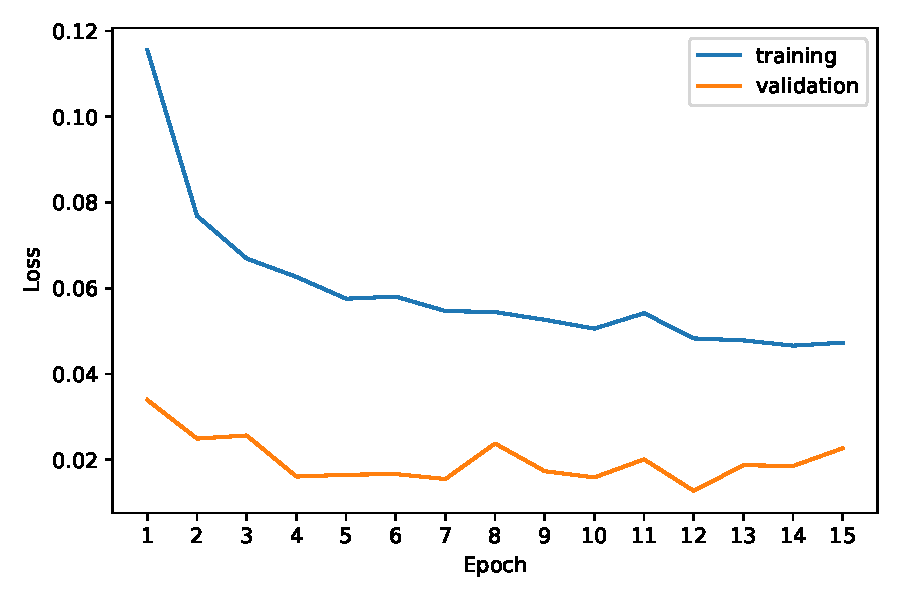
\includegraphics[width=0.7\textwidth]{abbildungen/training_plot}
    \caption[Trainings- und Validierungsverlust]{Wert der logistischen Verlustfunktion f\"ur Trainings- und Validierungsdatensatz
        innerhalb der ersten 15 Epochen.}
    \label{fig:training-loss}
\end{figure}

\subsubsection{Verarbeitung der Modellvorhersagen}

Um das Modell in der Pipeline einsetzen zu k\"onnen, muss aus den
Modellvorhersagen noch der Bereich extrahiert werden, welcher das
Nummernschild enth\"alt. Die hierzu eingesetzte Vorgehensweise
ist in Abbildung~\ref{fig:verarbeitung} anhand eines Beispielbildes
dargestellt.

\begin{figure}
    \begin{subfigure}{0.495\textwidth}
        \centering
        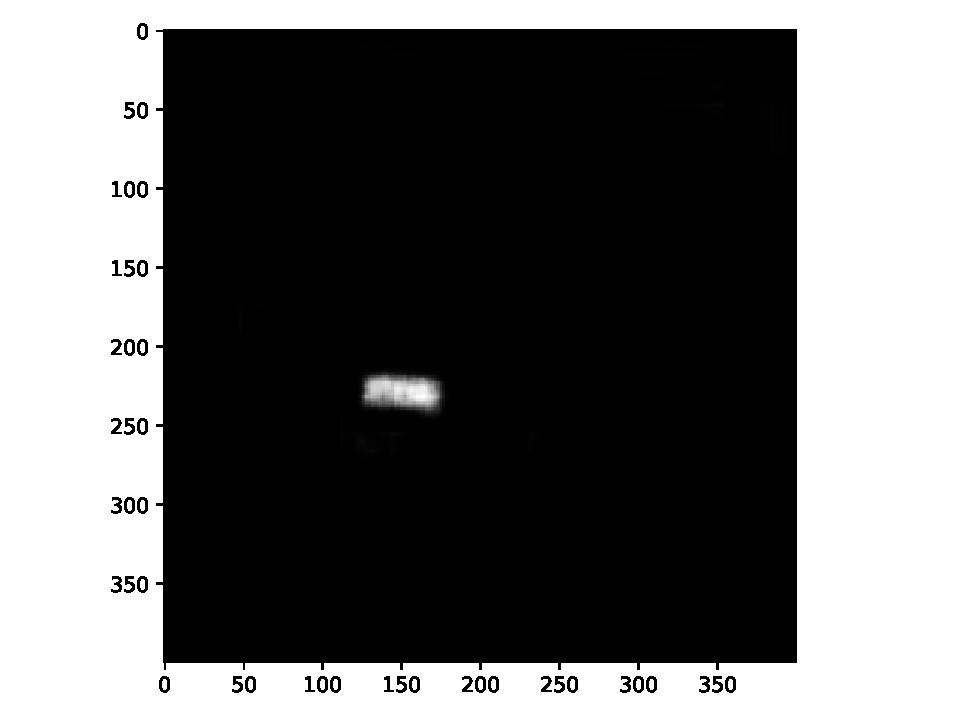
\includegraphics[width=\textwidth]{abbildungen/verarbeitung_1}
        \caption{Modellvorhersage}
    \end{subfigure}
    \begin{subfigure}{0.495\textwidth}
        \centering
        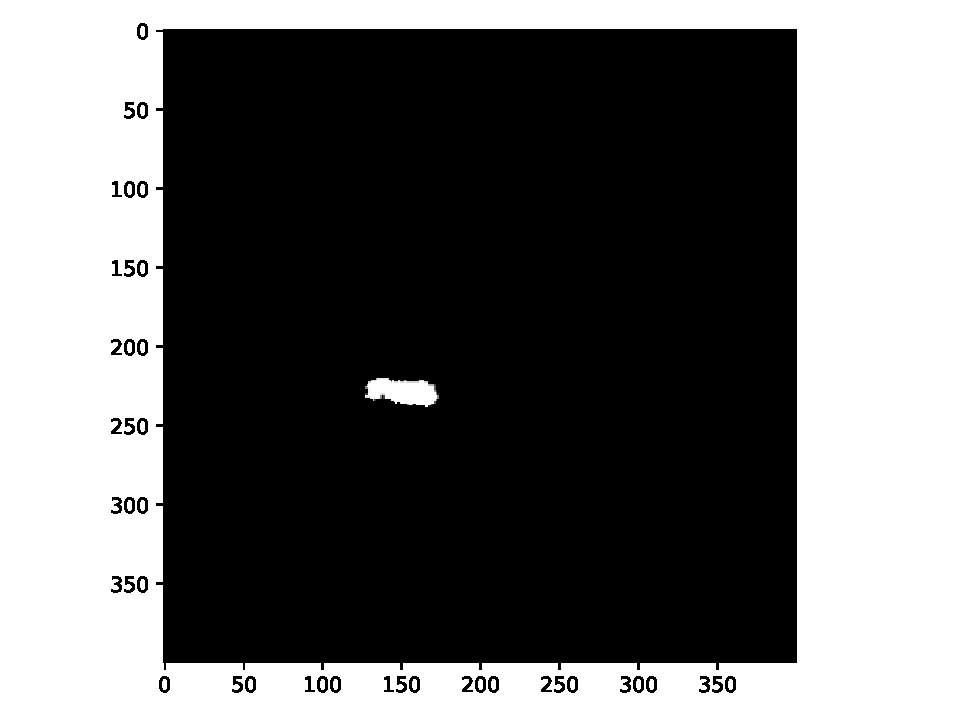
\includegraphics[width=\textwidth]{abbildungen/verarbeitung_2}
        \caption{Schwellenwert}
    \end{subfigure}
    \begin{subfigure}{0.495\textwidth}
        \centering
        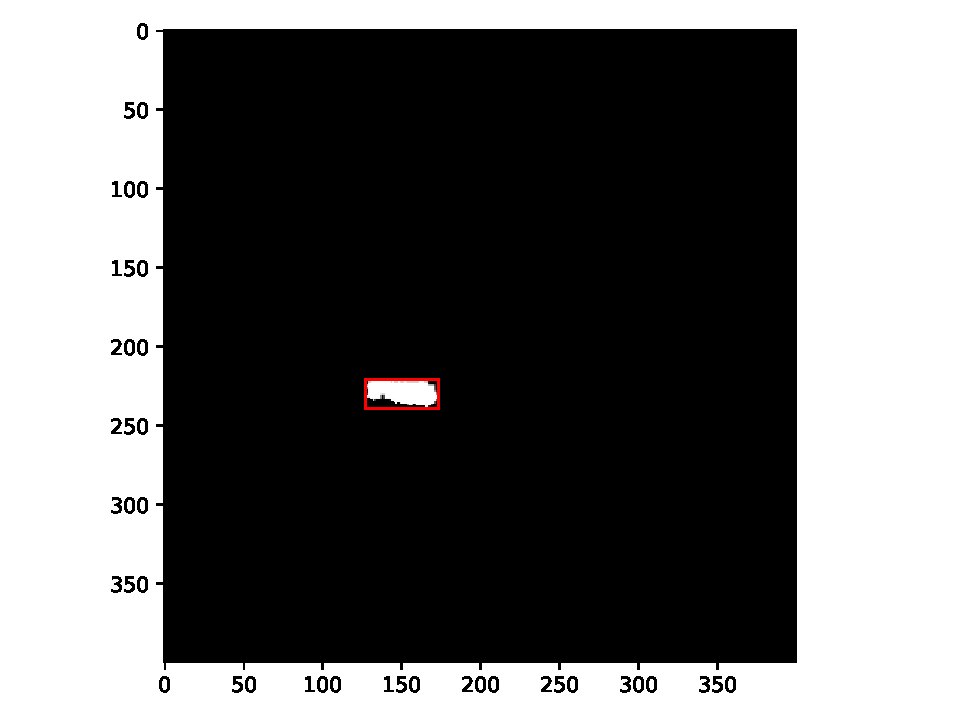
\includegraphics[width=\textwidth]{abbildungen/verarbeitung_3}
        \caption{Umschlie{\ss}endes Rechteck}
    \end{subfigure}
    \begin{subfigure}{0.495\textwidth}
        \centering
        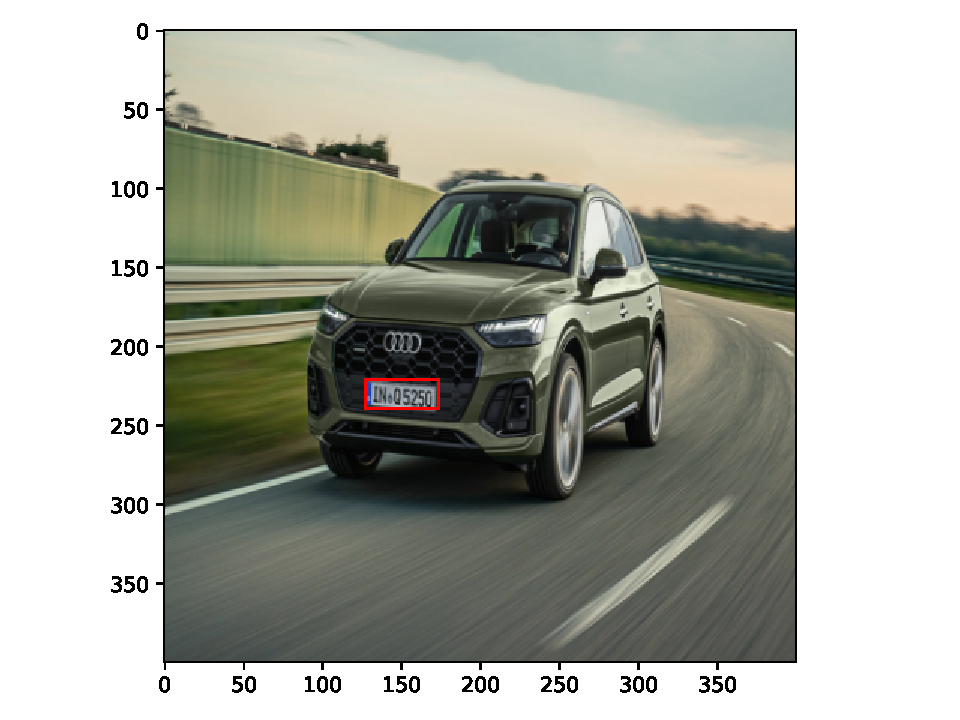
\includegraphics[width=\textwidth]{abbildungen/verarbeitung_4}
        \caption{Ergebnis}
    \end{subfigure}
    \caption[Verarbeitung der Modellvorhersage]{Verarbeitung der Modellvorhersage zur Extraktion des
        Nummernschildes. Das hier gezeigte Bild wurde weder zum Training
        noch zur Validierung w\"ahrend des Trainings verwendet.}
    \label{fig:verarbeitung}
\end{figure}

Der erste Schritt besteht darin, die Vorhersagen des Modells in eine
bin\"are Maske umzuwandeln, welche nur die Werte 1 und 0 enth\"alt
(1 f\"ur Pixel im Nummernschild, 0 f\"ur den Rest).
Da die Ausgabeschicht des eingesetzten Modells aufgrund der
Sigmoid-Funktion Werte im Intervall $[0, 1]$ ausgibt, wird
zu diesem Zweck (analog zur logistischen Regression)
ein Schwellenwertverfahren eingesetzt.
Hat ein Pixel in der Modellvorhersage einen Wert gr\"o{\ss}er als
0,5, so wird dieser in der bin\"aren Maske auf 1 gesetzt, alle
anderen Ausgaben werden auf 0 gesetzt.

Anschlie{\ss}end wird anhand der bin\"aren Maske ein rechteckiger
Ausschnitt bestimmt, in welchem das Nummernschild vermutet wird.
Dies geschieht so, dass zun\"achst f\"ur jeden zusammenh\"angenden
Bereich aus Einsen ein parallel zu den Koordinatenachsen
verlaufendes umschlie{\ss}endes Rechteck bestimmt wird.
Das fl\"achenm\"a{\ss}ig gr\"o{\ss}te dieser Rechtecke wird dann in
der Pipeline zur Extraktion des Nummernschildes verwendet.

Man beachte, dass hier implizit angenommen wird, dass sich
Nummernschilder stets durch ein parallel zur x- und y-Achse
verlaufendes Rechteck beschreiben lassen.
M\"ogliche Probleme mit diesem Ansatz, wie beispielsweise
rotierte Nummernschilder, liegen auf der Hand und werden sp\"ater
in Abschnitt~\ref{sec:ergebnisse} diskutiert.
Dennoch ist ein Vorteil dieses Ansatzes, dass er sehr leicht
umzusetzen ist und trotzdem, wie wir sp\"ater in
Abschnitt~\ref{sec:ergebnisse} sehen werden, zu guten Ergebnissen
f\"uhren kann.

\subsection{Texterkennung}
\label{sec:texterkennung}

Das Auslesen der Zeichen des Nummernschildes aus dem zuvor mithilfe des
CNN extrahierten Ausschnitt wurde mithilfe der
Optical Character Recognition (im Folgenden OCR) Software
Tesseract~\cite{tesseract} realisiert.

Damit Tesseract optimal arbeiten kann, werden zun\"achst
einige Vorverarbeitungsschritte durchgef\"uhrt, die in
Abbildung~\ref{fig:license-plate-preprocessing} dargestellt sind.
Hierbei wurde das Bild zun\"achst in Graustufen umgewandelt und
mit einem Weichzeichner gegl\"attet, um kleinere Unregelm\"a{\ss}igkeiten
und Bildrauschen zu entfernen.
Anschlie{\ss}end wurde auch hier ein Schwellenwertverfahren
eingesetzt, um die Zeichen klarer vom Hintergrund abzugrenzen.
Zur Bestimmung des Schwellenwertes kam Otsu's Methode~\cite{otsu} zum Einsatz,
die extra f\"ur eine
m\"oglichst klare Trennung von Vorder- und Hintergrund
entwickelt wurde. Im n\"achsten Schritt wurde das Bild dann
invertiert (Einsen wurden auf Nullen gesetzt und umgekehrt), um dann
die wei{\ss}en Bereiche, welche auch die zu erkennenden Zeichen
enthalten, zu erweitern (man spricht auch von Dilatation).
S\"amtliche dieser Schritte wurden mithilfe der
Computervision-Programmbibliothek OpenCV~\cite{opencv_library}
durchgef\"uhrt.

\begin{figure}
    \centering
    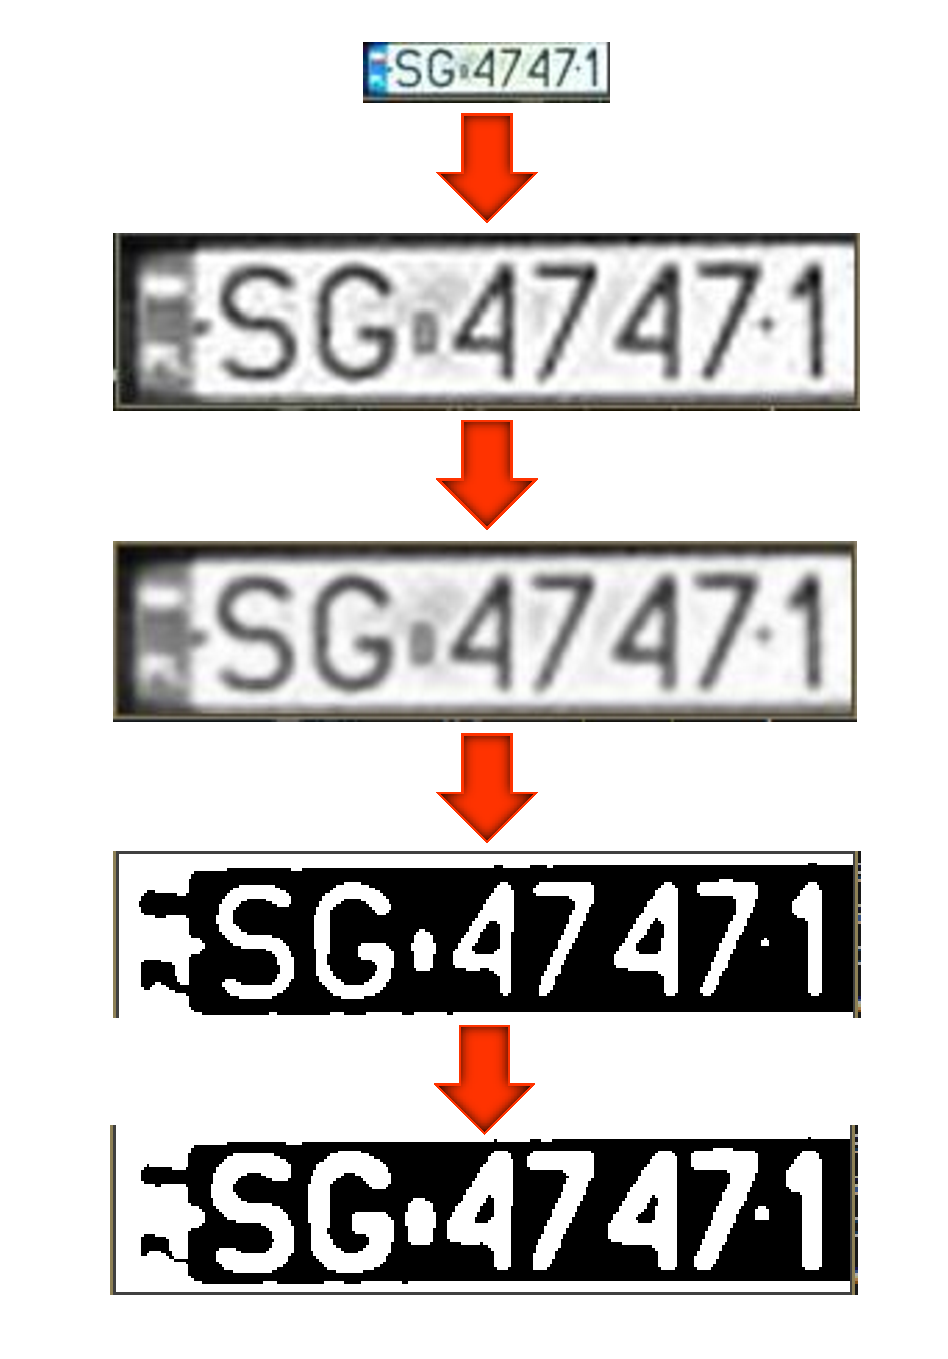
\includegraphics[width=0.35\textwidth]{abbildungen/license_plate_preprocessing}
    \caption[Vorverarbeitung eines Nummernschildes]{Die Vorverarbeitungsschritte
    eines Nummernschildes von oben nach unten aufgef\"uhrt:
    (1) Vergr\"o{\ss}erung und Umwandlung in Graustufen,
    (2) Bildgl\"attung,
    (3) Schwellenwert und Invertierung,
    (4) Dilatation}
    \label{fig:license-plate-preprocessing}
\end{figure}

F\"ur den Einsatz von Tesseract m\"ussen im n\"achsten Schritt noch die
einzelnen Zeichen ausgeschnitten werden.
Dies wurde mithilfe der automatisierten Konturenfindung
von OpenCV umgesetzt.
Die darauf folgenden Schritte der Pipeline sind in
Abbildung~\ref{fig:character-preprocessing} aufgef\"uhrt.
Die ausgeschnittenen Zeichen werden invertiert und anschlie{\ss}end
durch Tesseract erkannt.

\begin{figure}
    \centering
    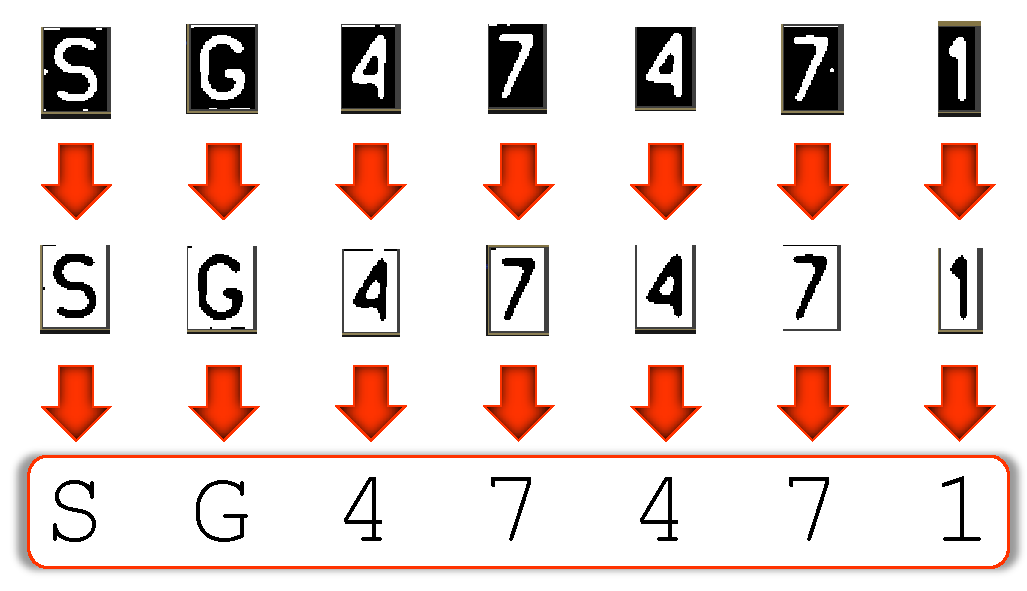
\includegraphics[width=0.5\textwidth]{abbildungen/character_preprocessing}
    \caption[Vorverarbeitung der einzelnen Zeichen]{Die ausgeschnittenen
        Zeichen werden wieder invertiert und dann durch
        Tesseract erkannt.}
    \label{fig:character-preprocessing}
\end{figure}